Para que nuestra smartTV sea capaz de usar Miracast sin necesidad de Chromecast necesitaría soportar Wi-Fi Direct, es decir, estuviera conectada por Wi-Fi y fuese compatible con ella.
Los dispositivos que envían y reciben información tienen que estar certificados para Miracast, pero existe un plug para dispositivos no certificados.
Miracast está disponible para dispositivos Android 4.2 o superior.

\vspace{0.1cm}
\begin{figure}[ht] 
	\begin{minipage}[b]{0.55\linewidth}
		La conexión está creada vía Wi-Fi Protected Setup (WPS), mecanismos para facilitar la configuración de una red WLAN con seguridad WPA2.
		WPS contempla cuatro configuraciones para el intercambio de credenciales, PIN (Personal Identification Number), PBC (Push Button Configuration), NFC (Near Field Communications) y USB (Universal Serial Bus). La configuración PIN no es recomendable por su debilidad ante ataques de fuerza bruta.
	\end{minipage}%%
	\begin{minipage}[b]{0.45\linewidth}
		\centering
		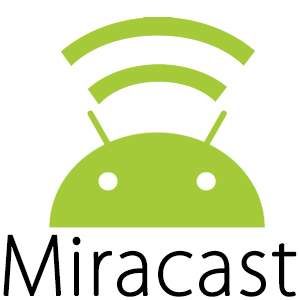
\includegraphics[width=.55\linewidth]{./Imagenes/miracast.jpg} 
	\end{minipage} 
\end{figure}

\begin{itemize}
	\item Capa de internet: IPv4
	\item Capa de transporte: TCP/UDP
	\item Capa de aplicación: RTSP y RTP controlan el streaming
\end{itemize}

A partir de Android 6.0 Google ha dejado de dar soporte a Miracast en favor de su propio Chromecast.
Con Miracast el dispositivo receptor es dependiente del dispositivo Android emisor\cite{Miracast}, si se bloquea también bloqueará la reproducción en el receptor. Esto puede ser una gran desventaja, por ejemplo, para la batería del emisor.

Chromecast solo necesita enviar la señal durante la configuración inicial, y en caso de querer parar la reproducción, subir/bajar volumen, etc., después se libera el emisor.
Chromecast no reproduce contenido protegido por Digital Rights Management (DRM).



\subsubsection{MiracleCast}
MiracleCast es una alternativa de código abierto a Miracast. El nombre viene por la dificultad de crear una red Wifi-P2P estable (basado en $wpa_supplicant$).

El núcleo de MiracleCast es un demonio llamado miracled \cite{MiracleCast}, que controla links locales, las peticiones de conexión, se encarga de
la codificación del protocolo y el parsing.
Su línea de comandos puede ser usada para controlar el demonio, crear nuevas conexiones, modificar parámetros, etc.
Soporta un modo interactivo que muestra las peticiones de conexión y permite al usuario aceptarlas o no.

El código fuente se puede encontrar en \href{https://github.com/albfan/miraclecast}{github}.